\uuid{Rs3w}
\exo7id{5464}
\titre{exo7 5464}
\auteur{rouget}
\organisation{exo7}
\datecreate{2010-07-10}
\isIndication{false}
\isCorrection{true}
\chapitre{Intégration}
\sousChapitre{Intégrale de Riemann dépendant d'un paramètre}
\module{Analyse}
\niveau{L2}
\difficulte{}

\contenu{
\texte{
\begin{itemize}
\item  Déterminer $\lim_{x\rightarrow 1}\int_{x}^{x^2}\frac{dt}{\ln t}$. 
\item  Etude complète de $F(x)=\int_{x}^{x^2}\frac{dt}{\ln t}$.
\end{itemize}
}
\reponse{
Si $x>1$, $[x,x^2]\subset]1,+\infty[$ et $t\mapsto\frac{1}{\ln t}$ est continue sur $]1,+\infty[$. Par suite, $\int_{x}^{x^2}\frac{dt}{\ln t}$ existe. De plus,

$$x\int_{x}^{x^2}\frac{1}{t\ln t}\;dt\leq\int_{x}^{x^2}\leq\int_{x}^{x^2}\frac{dt}{\ln t}=\int_{x}^{x^2}t\frac{1}{t\ln t}\;dt\leq x^2\int_{x}^{x^2}\frac{1}{t\ln t}\;dt.$$

Mais, 

$$\int_{x}^{x^2}\frac{1}{t\ln t}\;dt=\left[\ln|\ln t|\right]_{x}^{x^2}=\ln|\ln(x^2)|-\ln|\ln(x)|=\ln\left|\frac{2\ln x}{\ln x}\right|=\ln2.$$

Donc, $\forall x>1,\;x\ln2\leq F(x)\leq x^2\ln2$. On en déduit que $\lim_{x\rightarrow 1,\;x>1}F(x)=\ln2$.

Si $0<x<1$, on a $x^2<x$ puis $[x^2,x]\subset]0,1[$. Donc, $t\mapsto\frac{1}{\ln t}$ est continue sur $[x^2,x]$ et $F(x)=-\int_{x^2}^{x}\frac{1}{\ln t}\;dt$ existe.

Pour $t\in[x^2,x]$, on a $t\ln t<0$ et $x^2\leq t\leq x$. Par suite, 

$$x\frac{1}{t\ln t}\leq t\frac{1}{t\ln t}=\frac{1}{\ln t}\leq x^2\frac{1}{t\ln t},$$

puis, $\int_{x^2}^{x}x\frac{1}{t\ln t}\;dt\leq\int_{x^2}^{x}\frac{1}{\ln t}\;dt\leq\int_{x^2}^{x}x^2\frac{1}{t\ln t}\;dt$, et finalement,

$$x^2\ln2=\int_{x}^{x^2}x^2\frac{1}{t\ln t}\;dt\leq F(x)=\int_{x}^{x^2}\frac{1}{\ln t}\;dt\leq\int_{x}^{x^2}x\frac{1}{t\ln t}\;dt=x\ln 2.$$

On obtient alors $\lim_{x\rightarrow 1,\;x<1}F(x)=\ln2$ et finalement, $\lim_{x\rightarrow 1}F(x)=\ln2$. On en déduit que $F$ se prolonge par continuité en $1$ en posant $F(1)=\ln 2$ (on note encore $F$ le prolongement obtenu).
On a déjà vu que $F$ est définie (au moins) sur $]0,+\infty[$ ($F$ désignant le prolongement). Il ne parait pas encore possible de donner un sens à $F(0)$ et encore moins à $F(x)$ quand $x<0$, car alors $[x,0]$ est un intervalle de longueur non nulle contenu dans $[x,x^2]$, sur lequel la fonction $t\mapsto\frac{1}{\ln t}$ n'est même pas définie.

$$D_F=]0,+\infty[.$$

Pour $t\in]0,1[\cup]1,+\infty[$, posons $g(t)=\frac{1}{\ln t}$ et notons $G$ une primitive de $g$ sur cet ensemble. Alors, pour $x$ dans $]0,1[\cup]1,+\infty[$, $F(x)=G(x^2)-G(x)$. On en déduit que $F$ est dérivable (et même de classe $C^1$) sur $]0,1[\cup]1,+\infty[$ et que pour $x$ dans $]0,1[\cup]1,+\infty[$,

$$F'(x)=2xg(x^2)-g(x)=\frac{2x}{\ln(x^2)}-\frac{1}{\ln x}=\frac{x-1}{\ln x}.$$

Maintenant, quand $x$ tend vers $1$, $\frac{x-1}{\ln x}$ tend vers $1$. Ainsi, $F$ est continue sur $]0,+\infty[$, de classe $C^1$ sur $]0,1[\cup]1,+\infty[$ et $F'$ a une limite réelle en $1$. Un théorème classique d'analyse permet d'affirmer que  $F$ est de classe $C^1$ sur $D_F$ et en particulier, dérivable en $1$ avec $F'(1)=1$.

$$\forall x\in]0,+\infty[,\;F'(x)=\left\{
\begin{array}{l}
\frac{x-1}{\ln x}\;\mbox{si}\;x\neq1\\
1\;\mbox{si}\;x=1.
\end{array}
\right..$$

Si $x>1$, $x-1>0$ et $\ln x>0$ et si $0<x<1$, $x-1<0$ et $\ln x<0$. Dans tous les cas ($0<x<1$, $x=1$, $x>1$)  $F'(x)>0$. $F$ est strictement croissante sur $]0,+\infty[$.

On a vu que $\forall x>1,\;F(x)>x\ln2$ et donc $\lim_{x\rightarrow +\infty}F(x)=+\infty$. Plus précisément, pour $x>1$,

$$\frac{F(x)}{x}=\frac{1}{x}\int_{x}^{x^2}\frac{1}{\ln t}\;dt\geq\frac{x^2-x}{x\ln x}=\frac{x-1}{\ln x}.$$

Comme $\frac{x-1}{\ln x}$ tend vers $+\infty$ quand $x$ tend vers $+\infty$, on en déduit que $\frac{F(x)}{x}$ tend vers $+\infty$ quand $x$ tend vers $+\infty$ et donc que la courbe représentative de $F$ admet en $+\infty$ une branche parabolique de direction $(Oy)$.

Pour $x\in]0,1[$ et $t\in[x^2,x]$, on a $2\ln x=\ln(x^2)\leq\ln t\leq\ln x<0$ et donc $\frac{1}{\ln x}\leq\frac{1}{\ln t}\leq\frac{1}{2\ln x}$, puis $(x-x^2)\frac{1}{\ln x}\leq\int_{x^2}^{x}\frac{1}{\ln t}\;dt\leq(x-x^2)\frac{1}{2\ln x}$ et finalement,

$$\forall x\in]0,1[,\;\frac{x-x^2}{-2\ln x}\leq F(x)\leq\frac{x-x^2}{-\ln x}.$$

On obtient déjà $\lim_{x\rightarrow 0}F(x)=0$. On peut prolonger $F$ par continuité en $0$ en posant $F(0)=0$. Ensuite, $\frac{F(x)-F(0)}{x-0}=\frac{F(x)}{x}$ est compris entre $\frac{1-x}{-2\ln x}$ et $\frac{1-x}{-\ln x}$. Comme ces deux expressions tendent vers $0$ quand $x$ tend vers $0$, on en déduit que $\frac{F(x)-F(0)}{x-0}$ tend vers $0$ quand $x$ tend vers $0$. $F$ est donc dérivable en $0$ et $F'(0)=0$.

$$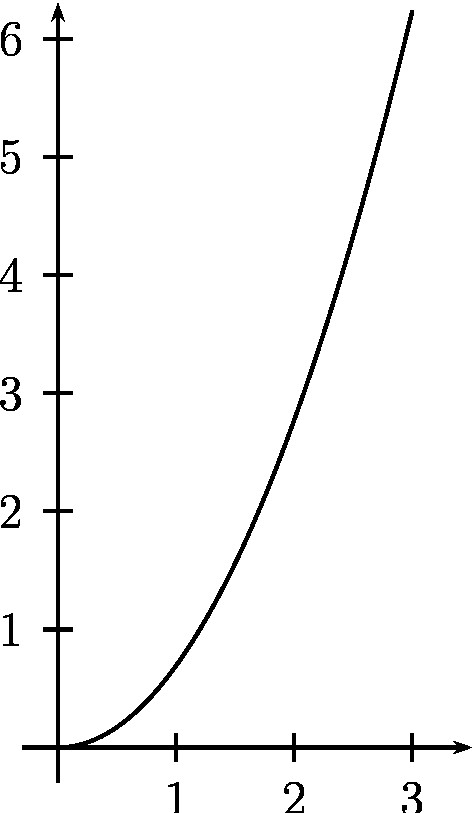
\includegraphics{../images/Rs3w-1}$$
}
}
